\documentclass[a4paper,USenglish,cleveref,autoref,thm-restate]{lipics-v2021}

\usepackage{isabelle}
\usepackage{isabellesym}
\isabellestyle{it}
% The italic style prints `_` as a hyphen; Isabelle names in the prose keep it.
\def\isacharunderscore{\_}
\usepackage{amssymb}
\usepackage{stmaryrd}
\usepackage{booktabs}
\usepackage{multirow}
\usepackage{tikz}
\usetikzlibrary{arrows.meta,positioning,fit,calc,backgrounds}

\setlength{\emergencystretch}{1.5em}
% Notation, one definition per concept. Mirrors thesis/lib/math.typ where the
% thesis has a symbol; the paper adds none the theories lack.

% Isabelle entities in prose: typewriter, never plain text.
% Breaks after underscores, so long names do not overrun the margin.
\makeatletter
\DeclareRobustCommand{\isaname}[1]{\texttt{\isa@split#1_\isa@end}}
\def\isa@split#1_#2\isa@end{#1\ifx\relax#2\relax\else\_\allowbreak\isa@split#2\isa@end\fi}
\makeatother
% A named obligation of the coverage contract.
\newcommand{\oblig}[1]{\textsc{#1}}
% Analyzer verdicts.
\newcommand{\verdict}[1]{\textsf{\small #1}}
% Trace constructors.
\newcommand{\ctor}[1]{\textsf{#1}}

% Semantic sets, as declared in the theories.
\newcommand{\Traces}{\mathcal{T}}
\newcommand{\NodeColl}{\mathcal{C}}
\newcommand{\ActColl}{\mathcal{A}}
\newcommand{\Report}{\mathcal{R}}
\newcommand{\Verd}{\mathcal{V}}
\newcommand{\Glob}{\mathcal{G}}
\newcommand{\cover}{\mathit{cover}}
\newcommand{\adm}{\mathit{adm}}
\newcommand{\conc}{\gamma}
\newcommand{\sol}{\sigma}

% Drafting markers; must be gone before submission.
\newcommand{\todo}[1]{\textcolor{red}{[TODO: #1]}} % chktex 13

% A generated Isabelle snippet, typeset small.
\newcommand{\snippet}[1]{{\small\input{generated/#1}}}

\input{generated/stats}
% latexmkrc defines the commit; a plain pdflatex run records none.
\providecommand\paperrevision{unknown}
\hypersetup{pdfinfo={Revision={\paperrevision}}}

\bibliographystyle{plainurl}

\title{End-to-End Soundness of a Context-Sensitive Goblint-Style Analyzer in Isabelle/HOL}
\titlerunning{End-to-End Soundness of a Goblint-Style Analyzer}

\author{Manuel Lerchner}{Technical University of Munich, Germany}{manuel.lerchner@tum.de}{}{}
\authorrunning{M. Lerchner}
\Copyright{Manuel Lerchner}

\ccsdesc[500]{Theory of computation~Program analysis}
\ccsdesc[300]{Theory of computation~Logic and verification}
\ccsdesc[300]{Software and its engineering~Formal software verification}

\keywords{abstract interpretation, interprocedural analysis, calling contexts,
  side-effecting constraint systems, verified static analysis, Isabelle/HOL}

\relatedversiondetails{Master's thesis and full formalization}{https://github.com/ManuelLerchner/Voblint-Verification-Master-Thesis}
\supplementdetails[subcategory={Isabelle/HOL formalization and analyzer}, cite=voblint]{Software}{https://doi.org/10.5281/zenodo.23260696}
\nolinenumbers

% Unpublished: no LIPIcs event, volume, or article number to claim yet.
\hideLIPIcs

\begin{document}

\maketitle

\begin{abstract}
Goblint-style analyzers solve side-effecting equations over shared global
unknowns and local unknowns indexed by program point and calling context.
An existing solver for these equations has been proved partially correct in
Isabelle/HOL, but its theorem does not connect the equations to source
execution. We mechanize this connection for a scalar imperative language
with recursive procedures, but without pointers or heap memory.

We adapt the local traces of Schwarz et al.\ to procedure activations,
retaining the caller that each return resumes. A relational context policy
specifies which contexts are admissible for each concrete call. We give five
local obligations on a cover and prove that, for any control-flow graph,
any cover satisfying them covers every valid trace's final store in every
admitted context. Post-solutions of the generated equations (valuations satisfying
their inequations) satisfy this contract when the context policy agrees
with the routing. The verified solver's certificate supplies such a
post-solution.

For every supported configuration, whenever the analyzer function exported
to OCaml returns a report, the report covers every store reached by a finite
source execution at its program point, and its definite verdicts hold for
those stores. This establishes partial correctness; solver termination
is not proved.
\end{abstract}


\section{Introduction}
\label{sec:intro}

A sound static analyzer over-approximates every execution of a program, so a
property that holds of the over-approximation holds in every run. The
guarantee is only as good as the analyzer's implementation, and analyzers are
large programs. Goblint, an abstract interpreter for C, has reported no false
negative on the SV-COMP benchmark suite since its first participation in
2021~\cite{seidl26}, yet its issue tracker lists more than a hundred issues
labeled as unsound in the same period. In one of them, the congruence domain
claimed \texttt{c \% 2 == 1} for $c \in \{-5, -7\}$, although C's truncating
remainder gives $-1$ for both values~\cite{goblint1161}. The defect (issue 1156) was reported only after Goblint had claimed the
false result.

A machine-checked proof rules out such defects for every input, but only if a
theorem connects the proved parts to the tool the user runs. For Goblint's
architecture, one part has been verified. Goblint translates a program into a
\emph{side-effecting constraint system}~\cite{seidl03,apinis12}, whose
right-hand sides may contribute to unknowns other than their own, and solves it
with a generic top-down solver. Stade et al.\ proved that solver partially
correct in Isabelle/HOL~\cite{stade24}, and Tilscher et al.\ extended the proof
to side effects~\cite{tilscher26}. When it terminates, the solver returns a post-solution on the unknowns it
solved, a set closed under the reads of right-hand sides. Whether those equations describe
the program lies outside the theorem.

Calling contexts make that missing link hard. A context-sensitive analysis
keeps one unknown per program point and calling context. Suppose
\texttt{main} calls \texttt{bump(5)} and \texttt{bump(4)}, and \texttt{bump}
returns its argument plus one. An analysis whose contexts record the argument
claims the result~6 in one context and~5 in the other. The collecting
semantics, the set of stores that executions bring to each program point,
holds both results at the return of \texttt{bump} but forgets which call
produced which store. A per-context claim therefore has nothing to be checked
against. Among mechanized analyzers, Dabrowski and Pichardie instrument a
concrete semantics with contexts, but their analysis is specified by
constraints that no solver computes~\cite{dabrowski09}. The other works we compare have no procedures, distinguish no contexts, or
reanalyze a function at each call site
(\cref{sec:related}).

We give calling contexts a concrete meaning and use it to verify a
Goblint-style analyzer end to end. The development, called Voblint, is written
in Isabelle/HOL and contains no \texttt{sorry}. Its contributions are:
\begin{itemize}
  \item \emph{A concrete semantics of calling contexts.} An \emph{activation
    trace} records one procedure activation together with the activation that
    created it, and a context policy relates each trace to the contexts it may
    carry. The relation may admit several contexts for one call. Under a
    totality condition, splitting the collecting semantics by context loses no
    store (\cref{sec:traces}).
  \item \emph{A soundness contract of five local obligations.} Any assignment
    of store sets to nodes and contexts that meets the obligations bounds every
    valid trace in every admitted context. The contract mentions no domain,
    equation, or solver (\cref{sec:traces}).
  \item \emph{A modular discharge of the contract.} Every post-solution of the
    generated, context-routed equations meets the contract. Domains, context
    policies, and the solver each prove their own obligations, and the solver
    enters only through its certificate (\cref{sec:equations}).
  \item \emph{An end-to-end theorem about the shipped analyzer.} Whenever the
    analyzer function returns a report, every store that a finite source execution from an initial store with zeroed
globals reaches is covered by the report and satisfies its definite verdicts, for
    every configuration the function offers. The function is the one exported
    to OCaml (\cref{sec:theorem}). Further theorems show that the result is
    not vacuous and that a domain obligation rejects the Goblint defect above
    (\cref{sec:evaluation}).
\end{itemize}
The solver, side-effecting constraint systems, the local traces that
activation traces adapt~\cite{schwarz21}, and the architecture of separating
analyses from solvers~\cite{vojdani16,seidl26} are prior work. Our
contribution is their connection: to our knowledge, no prior mechanization
leads from a source semantics through a context-indexed collecting semantics to
a side-effecting constraint system and its verified solver.

The guarantee has a precise scope. The source language, VIMP, has integer
variables, global variables, and recursive procedures with parameters and
return values, but no pointers, arrays, or heap. The result is partial
correctness: the analyzer answers only when its solver run terminates, and
termination is not proved for every program. The parser, Isabelle's code
generator, and the OCaml toolchain are trusted.

\section{Overview: One Call Through the Pipeline}
\label{sec:overview}

\begin{figure}[t]
\centering
\begin{minipage}[c]{0.27\textwidth}
\scriptsize
\begin{verbatim}
fun bump(n) {
  return n + 1;
}

fun main() {
  a = bump(5);
  b = bump(4);
  __voblint_check(a == 6);
  __voblint_check(b == 5);
}
\end{verbatim}
\end{minipage}%
\hfill
\begin{minipage}[c]{0.71\textwidth}
\centering
% Values: voblint --analysis interval --context entry-state --globals warrow
%         --dot docs/readme-figures/contexts.vimp
\resizebox{\linewidth}{!}{%
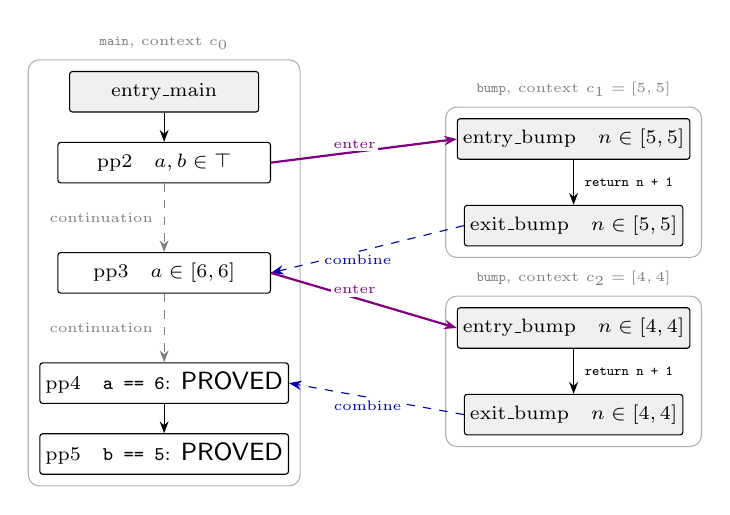
\begin{tikzpicture}[
  font=\scriptsize,
  pp/.style={draw, rounded corners=1pt, inner sep=2pt, minimum height=3.4ex, minimum width=27mm, align=left},
  bd/.style={pp, fill=black!6, minimum width=24mm},
  flow/.style={-{Stealth[length=1.5mm]}},
  call/.style={-{Stealth[length=1.6mm]}, thick, violet},
  ret/.style={-{Stealth[length=1.6mm]}, dashed, blue!70!black},
  lab/.style={font=\tiny, fill=white, inner sep=1pt}]
  \node[bd] (em) at (0, 0) {entry\_main};
  \node[pp] (p2) at (0, -0.9) {pp2\quad $a, b \in \top$};
  \node[pp] (p3) at (0, -2.3) {pp3\quad $a \in [6,6]$};
  \node[pp] (p4) at (0, -3.7) {pp4\quad \texttt{a == 6}: \verdict{PROVED}};
  \node[pp] (p5) at (0, -4.6) {pp5\quad \texttt{b == 5}: \verdict{PROVED}};
  \draw[flow] (em) -- (p2);
  \draw[flow, gray, dashed] (p2) -- node[lab, left=1mm] {continuation} (p3);
  \draw[flow, gray, dashed] (p3) -- node[lab, left=1mm] {continuation} (p4);
  \draw[flow] (p4) -- (p5);
  \begin{scope}[on background layer]
    \node[draw=gray!60, rounded corners, fit=(em)(p5), inner sep=4pt,
      label={[gray, font=\tiny]above:{\texttt{main}, context $c_0$}}] {};
  \end{scope}
  \node[bd] (b1e) at (5.2, -0.6) {entry\_bump\quad $n \in [5,5]$};
  \node[bd] (b1x) at (5.2, -1.7) {exit\_bump\quad $n \in [5,5]$};
  \draw[flow] (b1e) -- node[lab, right=1mm] {\texttt{return n + 1}} (b1x);
  \begin{scope}[on background layer]
    \node[draw=gray!60, rounded corners, fit=(b1e)(b1x), inner sep=4pt,
      label={[gray, font=\tiny]above:{\texttt{bump}, context $c_1 = [5,5]$}}] {};
  \end{scope}
  \node[bd] (b2e) at (5.2, -3.0) {entry\_bump\quad $n \in [4,4]$};
  \node[bd] (b2x) at (5.2, -4.1) {exit\_bump\quad $n \in [4,4]$};
  \draw[flow] (b2e) -- node[lab, right=1mm] {\texttt{return n + 1}} (b2x);
  \begin{scope}[on background layer]
    \node[draw=gray!60, rounded corners, fit=(b2e)(b2x), inner sep=4pt,
      label={[gray, font=\tiny]above:{\texttt{bump}, context $c_2 = [4,4]$}}] {};
  \end{scope}
  \draw[call] (p2.east) -- node[lab, above, pos=0.45] {enter} (b1e.west);
  \draw[ret] (b1x.west) -- node[lab, below, pos=0.55] {combine} (p3.east);
  \draw[call] (p3.east) -- node[lab, above, pos=0.45] {enter} (b2e.west);
  \draw[ret] (b2x.west) -- node[lab, below, pos=0.55] {combine} (p4.east);
\end{tikzpicture}} % chktex 31
\end{minipage}
\caption{The running example. Left: the VIMP program. Right: its graph as the
analyzer solves it with intervals and entry-state contexts. Each frame is one
procedure in one context; \texttt{bump} gets one copy per entry state. Solid
violet arrows are calls (enter), dashed blue arrows are returns (combine), and
dashed gray arrows link a call site to its continuation. Both checks are
\verdict{PROVED}. Without contexts, the single copy of \texttt{bump} joins both
calls and both checks are \verdict{UNKNOWN}. The states shown are analyzer
output using the warrowing update rule for global unknowns
(\cref{sec:equations}). The drawing omits the intermediate node of
\texttt{bump}'s body and the unreachable node after \texttt{return}.}
\label{fig:running}
\end{figure}

We follow the program of \cref{fig:running} through the analyzer, with
intervals and entry-state contexts. The source program is compiled to a
procedure-aware control-flow graph (CFG). Each procedure $p$ has an entry node
$\ctor{FunctionEntry}\;p$ and a result node $\ctor{FunctionResult}\;p$. The
graph $g$ has two kinds of edges. An \emph{intraprocedural} edge
$(u, a, v) \in \mathit{intra}\;g$ carries an action $a$, such as an
assignment or a guard. A \emph{call} edge
$(u, e, \ctor{FunctionEntry}\;p, k) \in \mathit{calls}\;g$ leads from the call
site $u$ into $p$ and names the continuation $k$ at which the caller resumes.
A predicate $\Glob$ tells which variables are global. A proved forward
simulation relates every source execution to a graph execution with the same
store (\cref{sec:theorem}).

From the graph, the analyzer generates inequations over \emph{local unknowns}
$(v, c)$ for a node $v$ and a context $c$, and over \emph{global unknowns}
without a program point. At \texttt{a = bump(5)}, the analysis's \emph{enter}
operation binds \texttt{n} to $[5,5]$, and this entry state is \emph{routed}
to the callee context $c_1 = [5,5]$; the second call routes to
$c_2 = [4,4]$. \Cref{sec:equations} gives the equations of a call. For these
two calls, the analyzer maintains separate context states and proves both
checks.

To interpret the abstract state in $c_1$, we need the concrete stores
associated with that context. Activation traces and a context policy define
this association (\cref{sec:traces}). The trace of the activation
\texttt{bump(5)} records its caller, the policy admits $c_1$ for that call, and
the \emph{activation collecting
semantics} $\ActColl(v, c)$ collects the final stores of the traces that end
at $v$ and carry $c$. The \emph{node collecting semantics} $\NodeColl(v)$
collects them regardless of context. An analyzer report $\mathit{res}$ defines
two sets at each node $v$. Its report set $\Report_{\mathit{res}}(v)$ is the
union of the stores represented by its abstract states at $v$ across all
contexts. The verdict set $\Verd_{\mathit{res}}(v)$ contains the stores in which
every definite verdict at $v$ holds: the check condition is true for
\verdict{PROVED} and false for \verdict{REFUTED}. Neither verdict asserts
reachability (\cref{sec:theorem}). The soundness argument is a chain of
inclusions at every node:
\begin{equation}
\label{eq:chain}
\text{reached stores}
\;\subseteq\; \NodeColl(v)
\;=\; \textstyle\bigcup_c \ActColl(v, c)
\;\subseteq\; \Report_{\mathit{res}}(v)
\;\subseteq\; \Verd_{\mathit{res}}(v).
\end{equation}
Each inclusion may add unreached stores, which costs precision, but none may
lose a reached store. The main end-to-end theorem
(\cref{sec:theorem}) states the outer inclusions, combining all contexts at
each node.

\section{Activation Traces and the Coverage Contract}
\label{sec:traces}

We adapt the local traces of Schwarz et al.~\cite{schwarz21} to procedure
activations. Context policies associate concrete calls with calling contexts,
following the use of call history by Sharir and Pnueli~\cite{sharir81}. We
formulate these policies as relations and introduce a coverage contract with
a soundness theorem. These definitions and the theorem are independent of
abstract domains, equations, and solvers.

For each node $v$ and context $c$, a context-sensitive analysis associates a set
intended to contain every store reached there in that context. To prove this
inclusion, we first define those concrete stores. A graph execution with a
plain frame stack does not record contexts: a frame holds only what is needed
to resume the caller and disappears at the return. Frames could carry a ghost context
(\cref{sec:mechanization}). We keep contexts out of the base trace semantics
and relate them to traces separately. Each call starts a new activation linked
to its caller; a return combines the completed callee trace with the caller
trace and resumes the caller.

\subsection{Activation traces}

An \emph{activation path} is the list of node--store pairs visited by one
activation. An activation trace has one constructor for each way an activation
begins or continues (\isaname{activation_trace}). $\ctor{Root}~\pi$ records
the activation of \texttt{main}. $\ctor{Call}~t'~\pi$ records a callee
activation and retains the caller trace $t'$ at the call site.
$\ctor{Resume}~t'~t''~\pi$ records the caller's continuation after the callee
trace $t''$ has completed. The observers $\mathit{path\_of}\;t$,
$\mathit{sink\_node}\;t$, and $\mathit{sink\_store}\;t$ return the path, its last
node, and its last store, respectively. The observer $\mathit{caller\_of}\;t$
returns the creating caller trace wrapped in $\mathit{Some}$, or
$\mathit{None}$ for the main activation. The operation
$\mathit{extend}\;t\;(v, s)$ appends a step to the path.

The datatype admits terms that no execution produces. The set
$\Traces_{\Glob,g,S}$ of \emph{valid} traces of a graph $g$ with initial stores
$S$, where $\mathit{entry}_g$ is the entry node of \texttt{main}, is defined
by four rules that mirror the rules of graph execution
(\isaname{valid_activation_trace}):
\begin{gather*}
\frac{s \in S}{\ctor{Root}\,[(\mathit{entry}_g, s)] \in \Traces}
\\[1ex]
\frac{t \in \Traces \quad (\mathit{sink\_node}\;t, a, v) \in \mathit{intra}\;g \quad s' \in \mathit{step}_a(\mathit{sink\_store}\;t)}{\mathit{extend}\;t\;(v, s') \in \Traces}
\\[1ex]
\frac{t \in \Traces \quad (\mathit{sink\_node}\;t, e, \ctor{FunctionEntry}\;p, k) \in \mathit{calls}\;g}{\ctor{Call}\;t\;[(\ctor{FunctionEntry}\;p,\; \mathit{enter}_e(\mathit{sink\_store}\;t))] \in \Traces}
\\[1ex]
\frac{\begin{array}{c}t'' \in \Traces \quad \mathit{caller\_of}\;t'' = \mathit{Some}\;t' \quad \mathit{sink\_node}\;t'' = \ctor{FunctionResult}\;p\\ (\mathit{sink\_node}\;t', e, \ctor{FunctionEntry}\;p, k) \in \mathit{calls}\;g\end{array}}{\ctor{Resume}\;t'\;t''\;\bigl(\mathit{path\_of}\;t' \mathbin{@} [(k, \mathit{combine}_e(\mathit{sink\_store}\;t', \mathit{sink\_store}\;t''))]\bigr) \in \Traces}
\end{gather*}
Here $\mathit{step}_a$ is the concrete meaning of an action, $\mathit{enter}_e$
binds the callee's formals to the call's arguments and resets its locals, and
$\mathit{combine}_e$ keeps the caller's locals, takes the callee's globals, and
assigns the return value to the call's destination (\isaname{combine_collect}).
A return resumes the activation identified by $\mathit{caller\_of}$.
The traces are defined for arbitrary graphs, so the return rule takes \emph{some} call edge from the caller's call site into $p$. It does
not require the edge through which the callee was entered. On compiled graphs
every call site has exactly one call edge (\isaname{calls_source_unique}), so
the two coincide.

Every finite source execution of a well-formed program yields a valid trace
that ends at the corresponding node with the same store, and whose chain of
callers represents the runtime frame stack
(\isaname{source_run_has_activation_trace}). The final stores of valid traces,
collected per node, form the node collecting semantics
$\NodeColl_{\Glob,g,S}(v)$ (\isaname{node_collect}).

In the local traces of Schwarz et al.~\cite{schwarz21}, $\ctor{Root}$
corresponds to an initial trace, $\ctor{Call}$ to thread creation, and
$\ctor{Resume}$ to the binary rule for acquiring a lock, which incorporates a
second trace (\cref{sec:related}).

\subsection{Calling contexts as a relation}

Call-string contexts record the last $k$ call sites; entry-state contexts
record the abstract values of the formals at entry. A \emph{context policy}
specifies which callee contexts a concrete call may belong to. It maps a call
site $u$, a caller context $c$, a description of the call, the caller's store,
and the entered store to the
\emph{set} of admitted callee contexts (\isaname{context_policy}). The result
is a set because Goblint's enter may return several
alternatives for one call, each routed separately. The set may be empty, for instance at a
call the analysis considers unreachable. The supplied analyses return a single
entry alternative, so a call is admitted in at most one context per caller
context. A Sign-analysis instance demonstrates the relational case: its enter
returns two overlapping alternatives, the plain entry state and one that
forgets the formals. One concrete call is then admitted in two contexts
(\isaname{ov_two_contexts_admitted}).

For a call edge $e$ into $p$, we write $\adm_{u,c}(e, s, s')$ for the set the
policy returns for the call described by $e$ and $p$, caller store $s$ and
entered store $s'$. We write $c' \in \adm^{\exists}_{u,c}(p, s, s')$ when some call edge from $u$
into $p$ maps $s$ to the entered store $s'$ and the policy admits $c'$ for it
(\isaname{admits_call_context}). The contexts a trace carries are then defined
inductively (\isaname{activation_context_rel}):
\begin{gather*}
\frac{}{\ctor{Root}\;\pi \text{ carries } c_0}
\qquad
\frac{t' \text{ carries } c}{\ctor{Resume}\;t'\;t''\;\pi \text{ carries } c}
\\[1ex]
\frac{t \text{ carries } c \quad c' \in \adm^{\exists}_{\mathit{sink\_node}\,t,\,c}(p, \mathit{sink\_store}\;t, s')}{\ctor{Call}\;t\;((\ctor{FunctionEntry}\;p, s') \mathbin{\#} \pi) \text{ carries } c'}
\end{gather*}
That is, the root carries the initial context $c_0$, a callee carries every
context admitted for its call from some context of its caller, and a resumed activation keeps the contexts it had
before the call. Traces store no context, so the policy is a parameter of
every theorem below. The activation collecting semantics collects the final
stores of the valid traces that end at $v$ and carry $c$
(\isaname{activation_collect}):
\[
\ActColl_{\Glob,\adm,c_0,g,S}(v, c) \;=\; \{\, \mathit{sink\_store}\;t \mid t \in \Traces_{\Glob,g,S},\; \mathit{sink\_node}\;t = v,\; t \text{ carries } c \,\}.
\]
In the running example, the final store of \texttt{bump(5)} lies in
$\ActColl(\ctor{FunctionResult}\;\texttt{bump}, [5,5])$ and that of
\texttt{bump(4)} in $\ActColl(\ctor{FunctionResult}\;\texttt{bump}, [4,4])$,
whereas $\NodeColl$ at that node contains both.

\subsection{The coverage contract}

A \emph{cover} assigns a set of stores to each node and context. The four
rules for valid traces give rise to four preservation obligations on a cover.
A fifth obligation ensures that each call from a covered store is admitted in
at least one context. We express this contract in the locale
\isaname{activation_coverage}; an Isabelle locale packages named parameters and
assumptions~\cite{ballarin14}. The obligations are as follows, with the call obligations
quantified over every call edge $(u, e, \ctor{FunctionEntry}\;p, k)$:
\begin{align*}
  &\oblig{Init} && s \in S \implies s \in \cover(\mathit{entry}_g, c_0)\\
  &\oblig{Intra} && (u, a, v) \in \mathit{intra}\;g,\; s \in \cover(u, c),\; s' \in \mathit{step}_a(s) \implies s' \in \cover(v, c)\\
  &\oblig{Call} && s \in \cover(u, c),\; c' \in \adm_{u,c}(e, s, \mathit{enter}_e(s))\\
  &&&\quad \implies \mathit{enter}_e(s) \in \cover(\ctor{FunctionEntry}\;p, c')\\
  &\oblig{Return} && s \in \cover(u, c),\; c' \in \adm^{\exists}_{u,c}(p', s, s'),\\
  &&&\quad t \in \cover(\ctor{FunctionResult}\;p, c') \implies \mathit{combine}_e(s, t) \in \cover(k, c)\\
  &\oblig{Total} && s \in \cover(u, c) \implies \adm_{u,c}(e, s, \mathit{enter}_e(s)) \neq \emptyset
\end{align*}
\oblig{Return} ranges over every procedure $p'$ and entered store $s'$
admitted at the call site. As in the return rule, the call edge $e$ used to
resume the caller can differ from the edge used to enter the callee. On a
graph with one call edge per call site, $p' = p$ and both operations use the
same edge.

If no context admits a call from a covered store, \oblig{Call} and
\oblig{Return} hold vacuously. They therefore do not ensure that the cover at
the continuation includes the returned store, even though the resumed caller
still carries its contexts there. Without \oblig{Total}, a cover that meets the
other four obligations can miss a reached store
(\isaname{total_dropped_unsound}). \oblig{Total} asks only about covered
stores, because an entry-state policy admits no context for stores the
analysis has excluded. Call strings and the unit policy, which admits one
context for every activation, meet it for every cover
(\isaname{call_context_total_on_of_fun}).

\begin{theorem}[Context-indexed soundness, \isaname{activation_collect_sound}]
\label{thm:contract}
If a cover meets the five obligations of \isaname{activation_coverage}, then
$\ActColl(v, c) \subseteq \cover(v, c)$ for every node $v$ and context $c$.
\end{theorem}

\subparagraph*{Proof idea.}
The proof is an induction over valid traces with the invariant that a trace
carries some context and that its final store is covered in every context it
carries. A single-trace invariant does not suffice for the return rule, which
needs the invariant for the caller recovered through $\mathit{caller\_of}$.
The induction therefore carries the invariant along the whole chain of
callers (\isaname{caller_chain_covered}, an instance of the induction
principle \isaname{caller_chain_closure}).

\oblig{Total} is used twice. In the call case, it supplies a context for the
new callee. In the return case, it supplies an admitted callee context $c'$
for each context $c$ of the resumed caller, using the callee's own entry edge.
The callee then carries $c'$ (\isaname{activation_context_rel_caller_entryI}),
so its exit store is covered at $c'$. \oblig{Return} ensures that combining
the caller store and callee exit store yields a store in the cover at the
continuation in context $c$. This is why \oblig{Return} ranges over the admitted
entry ($p'$, $s'$), which can differ from the entry specified by the call edge used for resumption.

Under the contract, every valid trace therefore carries at least one context,
so taking the union over contexts recovers the node collecting semantics
(\isaname{node_collect_eq_Union_activation_collect}):
\[
\NodeColl(v) \;=\; \textstyle\bigcup_c \ActColl(v, c).
\]

\section{From Equations to a Cover}
\label{sec:equations}

The contract of \cref{sec:traces} asks for a cover. This section constructs one
from a solved equation system. The ingredients have different origins. The
analysis interface mirrors Goblint's \texttt{Spec}~\cite{vojdani16,seidl26}.
Side-effecting equations come from Seidl et al.\ and Apinis
et al.~\cite{seidl03,apinis12}. The solver and its certificate are those of
Tilscher et al.~\cite{tilscher26}. The routing conditions, which connect the
equations to the context policy, and their discharge for each policy are ours.

\subsection{What an analysis supplies}

An analysis describes the stores at a node by an abstract state $d$. Its
meaning $\conc(d, \rho)$ also depends on $\rho$, the solved values of the
analysis's global unknowns. We suppress $\rho$ when it plays no role. The
analysis supplies the record \isaname{dg_spec}, the counterpart of Goblint's
\texttt{Spec}: one transfer per kind of edge action, an enter operation, and
two combine operations. A call needs two states. After the return, the
caller's locals come from before the call, while the globals and the result
come from the callee. Enter therefore returns a list of entry pairs $(q, e)$:
a resume state $q$ that describes the caller's store, and an entry state $e$
that describes the store in which the callee starts. Combine builds the state
after the call from $q$ and the callee's exit state.

The local soundness laws form the locale \isaname{analysis_contract}. The
concretization is monotone, every transfer loses no successor store, and
combine covers $\mathit{combine}_e(s, t)$ whenever $q$ covers $s$ and the exit
state covers $t$. In addition, enter must return a pair that covers the
caller's store and the entered store (\isaname{entry_pairs_cover}). A numeric
domain proves only its abstract operations sound. The framework derives the
transfers once for all domains, following Nipkow and Klein's generic
interpreter~\cite[Sect.~13.5]{nipkow14}. The shipped domains are Sign,
Interval, Parity, Congruence, and their reduced product.

\subsection{Context-indexed equations and routing}

For every node $v$ and context $c$ there is a local unknown $(v, c)$. Its
right-hand side joins four sources (\isaname{routed_node_rhs_parts}):
\begin{itemize}
  \item the initial state at the program entry;
  \item the transfer along each intraprocedural edge into $v$, in the same
    context $c$;
  \item the combined result of each call returning to $v$;
  \item at a procedure entry, the entry states published to it.
\end{itemize}
At a call, a \emph{routing function} chooses the callee context from the call
site, the caller context, and the entry state. Each call publishes its entry
state as a side effect to a global seed unknown for the callee and the chosen
context, which the callee's entry equation reads. A recursive call needs no
special treatment: its equation reads an exit state that depends on the
caller's own unknowns, and the solver handles the cycle as it handles a loop.

The equations choose a callee context from an abstract state, while the
concrete semantics chooses one from the concrete call through the policy
$\adm$. Two conditions make the choices agree. Both are assumptions of the
locale \isaname{routed_context}.
\begin{description}
  \item[Adequacy] (\isaname{routing_adequate}). If $\adm$ admits $c'$ for a call
    from a store that the caller's solved state describes, then enter produces
    a pair $(q, e)$ that is routed to $c'$, whose resume state covers the
    caller's store and whose entry state covers the entered store. The
    callee's entry unknown in $c'$ is solved.
  \item[Totality] (\isaname{routing_total}). $\adm$ admits at least one context
    for every call from a store that the caller's solved state describes.
\end{description}
For the unit policy and for call strings, $\adm$ admits exactly the context the
routing function computes from the call site and the caller context. Totality
is then immediate, and adequacy reduces to entry coverage and the routed entry
unknown being solved.

For entry-state contexts, the policy \isaname{routed_entry_context_rel} is
defined from the solved valuation $\sol$:
\begin{multline*}
\adm_{u,c}(e, s, s') \;=\; \{\, \mathit{route}(u, c, e') \mid {}\\
(q, e') \in \mathit{enter}(\sol(u, c)),\; s \in \conc(q),\; s' \in \conc(e') \,\}.
\end{multline*}
That is, a context is admitted when an entry pair of the solved caller state
covers both concrete stores and is routed there. The definition is not
circular. $\sol$ is fixed before the policy is applied, and the final
guarantee concerns $\NodeColl$, which no policy changes. The policy only
decides how $\NodeColl$ is split among contexts inside the proof. The
construction resembles the a posteriori soundness of Might and Manolios,
whose abstraction maps can only be built after the analysis has
run~\cite{might09}. In our case the abstraction is fixed in advance, and the
solution fixes the relation between traces and contexts. A consequence
matters for reading the result: under entry-state contexts, $\ActColl(v, c)$
is relative to the analysis that produced $\sol$.

\begin{table}[t]
\centering
\small
\begin{tabular}{@{}lp{0.6\textwidth}@{}}
\toprule
Hypothesis & Reading \\
\midrule
\texttt{analysis\_contract} & transfers, enter and combine are sound \\
\texttt{pp} (\texttt{post\_bounded}) & $\sol$ bounds every right-hand side on the solved set $V$ \\
\texttt{fwd} & an intraprocedural edge from a solved unknown with a non-empty state leads to a solved unknown \\
\texttt{comb\_fwd} & a call's continuation is solved in the caller's context \\
\texttt{routing\_adequate}, \texttt{routing\_total} & the policy agrees with the routing \\
\texttt{resolve\_sound} & callee resolution lists every procedure a covered store can call \\
\texttt{calls\_unique} & each call site has one call edge (\isaname{calls_source_unique}) \\
\texttt{is\_bot\_sound} & a state classified as bottom describes no store, so skipping its call is sound \\
\texttt{finC}, \texttt{finE} & the graph has finitely many edges \\
seed keys & seed unknowns differ from all other global unknowns \\
\bottomrule
\end{tabular}
\caption{Hypotheses of \cref{thm:routed}: the assumptions of the locales
\isaname{routed_context} and \isaname{dg_context_activation}. The theorem adds
that the program entry is solved in $c_0$ and that the initial state describes
the initial stores.}
\label{tab:hypotheses}
\end{table}

\begin{theorem}[Routed collecting soundness, \isaname{activation_collect_dg_sound}]
\label{thm:routed}
Under the hypotheses of \cref{tab:hypotheses}, if the program entry is solved
in context $c_0$, the initial state describes the initial stores under the
initial values of the global unknowns, and those values lie below the solved
ones $\rho$, then
$\ActColl(v, c) \subseteq \cover(v, c)$ for all $v$ and $c$, where
$\cover(v, c) = \conc(\sol(v, c), \rho)$ on solved unknowns and $\emptyset$
elsewhere.
\end{theorem}

The proof checks the five obligations of \cref{thm:contract} for this cover.
The initial state gives \oblig{Init}. The edge transfers and \texttt{fwd} give
\oblig{Intra}. Adequacy with entry coverage gives \oblig{Call}, adequacy with
combine soundness gives \oblig{Return}, and totality gives \oblig{Total}.
\oblig{Return} is quantified over every admitted call edge from the call site
(\cref{sec:traces}), and \texttt{calls\_unique} reduces it to the edge being
returned through.

\subsection{The solver enters through one certificate}

\Cref{thm:routed} needs a post-solution on a set of unknowns that contains the
program entry and is closed under execution steps. The verified top-down
solver~\cite{tilscher26} provides a different certificate,
\isaname{part_post_solution}, for the query $x$ it started on, its solved set
$V$, and its result $\sol$:
\snippet{part_post_solution}
\noindent Here $\sigma(\mathit{Inl}\;u)$ is the value of a local unknown $u$;
global unknowns are the $\mathit{Inr}$ side of the sum. That is, the query is
solved, $V$ is closed under the reads of right-hand sides, and $\sol$ bounds
both the right-hand side and every side effect of each solved unknown. The two certificates point in different
directions. The solver works backward from its query, the result of
\texttt{main}, while \cref{thm:routed} follows executions forward from the
entry. The bridge restricts $V$ to its \emph{live} part: the unknowns
$(u, c)$ such that $u$ belongs to a procedure $q$ whose result
$(\ctor{FunctionResult}\;q, c)$ is solved (\isaname{live_unknowns}). The
compiler ends every body with a return edge, so every node of a procedure
reaches the procedure's result through intraprocedural edges and
call-to-continuation steps. Closure under reads then puts all nodes of a
procedure into $V$ once its result is solved in that context.
\isaname{live_unknowns_cover} proves, from a well-formed program and a
returned solve, that the live set contains the program entry and is closed
forward. This is structural reachability in the graph. It does not claim
that an execution reaches the result. Three sets are involved: the solver's
solved set $V$, its live subset, on which \cref{thm:routed} is applied, and the
states the report publishes, which are taken from $V$. Publishing more
states than the proof uses is sound, because the report only has to contain
the cover.

The rest of the proof never inspects the solver. The analysis locale takes the
solver as a parameter and assumes four facts about it
(\isaname{certified_solver}): a run in its domain yields
\isaname{part_post_solution} and a finite solved set, and a run of its
executable form that returns lies in the domain and agrees with the logical
solver. These facts are proved for the vendored solver under each of its five
update rules for global unknowns (\isaname{td_certified_solver}). An update
rule decides how contributions to a global unknown accumulate: by join, by
join per contributing right-hand side, or by \emph{warrowing}, which combines
widening and narrowing~\cite{tilscher26}. Replacing the solver would not touch
the semantic layer.

\section{The End-to-End Theorem}
\label{sec:theorem}

The solved valuation bounds the context-indexed collecting semantics of the
CFG\@. A forward simulation connects source and graph executions, following
the CompCert methodology~\cite{leroy09}. Report construction then preserves
coverage and gives sound verdicts.

\subparagraph*{From source to graph.}
VIMP has a small-step semantics \isaname{pstep} over configurations
$(r, s, \mathit{frs})$ of a residual command (the code left to execute), a
store, and a frame stack. A
call pushes a frame holding the caller's store and destination and continues
with the callee's body followed by a $\mathit{Restore}$ marker; the marker pops
the frame and combines the stores as in \cref{sec:traces}
(\isaname{pstep}, rules \texttt{Call} and \texttt{RestoreStep}). A call whose
arity does not match, or whose callee is undeclared, is stuck; well-formedness
excludes such programs.

The compiler uses continuations to translate each procedure body into a
procedure-aware CFG\@. A forward simulation matches each source step with graph
steps that reach the same store (\isaname{csim_star}).

A source configuration does not determine a graph node. The residual command can occur in both branches of
\texttt{if (b) \{x = 1;\} else \{x = 1;\}}. The proof therefore annotates every
command of the program with its nodes. The relation
$p, s_0 \vdash (r, s, \mathit{frs}) \rhd v$ (\isaname{at_node}) holds when some
run of the annotated program from $s_0$ reaches an annotated configuration
that erases to $(r, s, \mathit{frs})$, names $v$, and is related to $v$ by the
simulation. In the example, the configuration after either branch is
observed at both branch nodes. The theorem quantifies over every node at which
a configuration is observed.

Combining the simulation with the result of \cref{sec:traces} shows that every
store reached by a finite source execution lies in $\NodeColl$ at a node
related to that execution (\isaname{source_reaches_node_collect}). For the
annotated program, this holds at every node where the execution is observed
(\isaname{csim_point_compile_prog}).

\subparagraph*{From valuation to report.}
The analyzer function \isaname{run_voblint} takes a configuration and a
program. The configuration selects the analyses, the update rule for global
unknowns, the context policy and call-string length, and the placement of
program globals. The function rejects an invalid
configuration or an ill-formed program, and otherwise runs the executable
solver and returns $\ctor{Analysed}~\mathit{res}$ when the solver returns a
result (\isaname{run_voblint}). At each node, the report lists the states
computed for its solved contexts and classifies each check as
\verdict{PROVED}, \verdict{REFUTED}, \verdict{UNKNOWN} (undetermined), or
\verdict{DEAD} (unreachable). The sets $\Report_{\mathit{res}}(v)$ and
$\Verd_{\mathit{res}}(v)$ interpret these states and verdicts as in
\cref{sec:overview}.

In the Isabelle statement below, \texttt{fixes} declares typed parameters,
\texttt{defines} introduces abbreviations, \texttt{assumes} lists premises,
and \texttt{shows} gives the conclusion. Here $\Pi$ is the procedure table of $p$, and
$\Glob, \Pi \vdash (c, s, \mathit{frs}) \rightarrow_p^* (c', s', \mathit{frs}')$
is a finite execution of \isaname{pstep} from residual command $c$, store $s$
and frame stack $\mathit{frs}$. $\NodeColl_{\Glob,g,S}\,v$ is the node
collecting semantics of the compiled graph $g$ from the initial stores $S$.

\begin{theorem}[End-to-end soundness, \isaname{run_voblint_source_sound}]
\label{thm:headline}
\end{theorem}
\vspace{-1.5ex}
\snippet{run_voblint_source_sound}

The theorem assumes an initial store with zero-valued globals and
unconstrained locals, a finite execution from the body of \texttt{main}, and a
returned analyzer report. This includes finite prefixes of nonterminating executions. The reached
configuration is observed at some node; at every such node, its store is
collected, covered by the report, and consistent with every definite verdict.
The proof combines contexts using $\NodeColl(v) = \bigcup_c \ActColl(v, c)$
and \cref{thm:routed}.

Under the configured policy, the report's states for $c$ at $v$ also cover
$\ActColl(v,c)$ (\isaname{run_voblint_context_covers}). The underlying
\isaname{run_voblint_contexts} theorem additionally ensures that every valid
activation trace has an admitted context.

A returned report entails solver termination, program well-formedness, and
coverage via \isaname{live_unknowns_cover}. No separate premises
restrict the accepted configurations.

\subparagraph*{Meaning of verdicts.}
\verdict{PROVED} states that whenever a covered execution reaches the check,
the condition holds; \verdict{REFUTED} that it fails
(\isaname{run_voblint_check_sound}). Neither asserts that the check is
reachable, and \verdict{REFUTED} is not a verified counterexample.
\verdict{DEAD} establishes that the check's node is unreachable (\isaname{run_voblint_dead_check_unreached}). Analogous theorems cover
arithmetic diagnostics. If a node has no diagnostic, divisors in its outgoing
edge expressions and call arguments are nonzero in every collected store
(\isaname{run_voblint_arithmetic_safe}). An error diagnostic establishes
that its divisor is zero in every collected store at that node
(\isaname{run_voblint_arithmetic_refuted}).

\subparagraph*{Trusted components.}
\Cref{fig:trust} separates what is proved from what is trusted. The theorem is
about the constant that Isabelle's code generator~\cite{haftmann10} exports to
OCaml and that the command-line tool calls. The lexer and parser, which
construct the program, and the handwritten OCaml that prints the report lie
outside the proof. The Isabelle kernel, the code generator, the OCaml
toolchain, and the arbitrary-precision integer library Zarith are trusted.
When tracing is requested, the command-line tool calls
\isaname{run_voblint_traced}, which is equal to \isaname{run_voblint} in
Isabelle (\isaname{run_voblint_traced_eq}). Its exported code maps
\isaname{trace_event}, whose logical result is the unit value $()$, to the
handwritten hook \texttt{Solver\_trace\_hook.emit}. The solver, routing
functions, and report construction call this hook. The traced executable
additionally trusts it to return without exceptions and leave the computed
results unchanged; untraced runs do not call it.

We must also justify that \isaname{pstep} models the intended language; the
soundness theorem does not establish this. Some of VIMP's choices differ
from C. Integers are unbounded. Division by zero
yields $0$ and the remainder by zero yields the dividend. Expressions are pure and
total, so operand evaluation order does not affect the values of
\texttt{\&\&} and \texttt{||}. A failed check does not stop
the execution, so a verdict for one check does not depend on an earlier one.
The locals of \texttt{main} start unconstrained, while a callee's locals start
at $0$. \texttt{min}, \texttt{max}, and the nondeterministic input are
built-in calls, and \texttt{main} has no explicit \texttt{return}. A verdict therefore does not always hold for a C program with the
same text.

\begin{figure}[t]
\centering
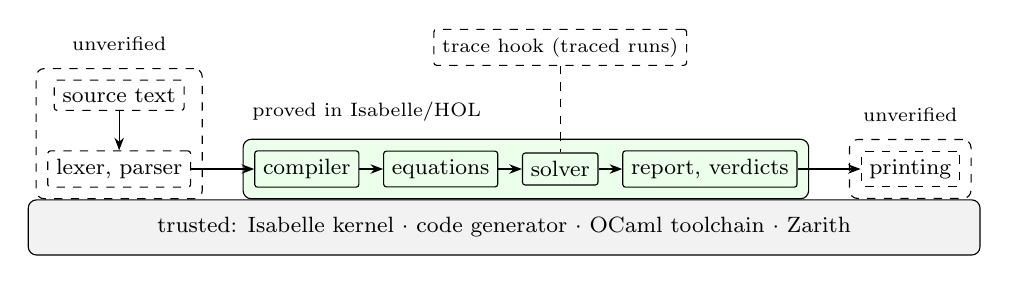
\begin{tikzpicture}[
  font=\footnotesize,
  part/.style={draw, rounded corners=1pt, align=center, inner sep=3pt},
  zone/.style={draw, rounded corners=3pt, inner sep=4pt},
  arr/.style={-{Stealth[length=1.6mm]}}]
  \node[part, dashed] (par) {lexer, parser};
  \node[part, dashed, above=5mm of par] (src) {source text};
  \node[part, right=8mm of par] (cmp) {compiler};
  \node[part, right=3mm of cmp] (eqs) {equations};
  \node[part, right=3mm of eqs] (slv) {solver};
  \node[part, right=3mm of slv] (rep) {report, verdicts};
  \node[part, dashed, right=8mm of rep] (out) {printing};
  \draw[arr] (src) -- (par); \draw[arr] (par) -- (cmp); \draw[arr] (cmp) -- (eqs);
  \draw[arr] (eqs) -- (slv); \draw[arr] (slv) -- (rep); \draw[arr] (rep) -- (out);
  \begin{scope}[on background layer]
    \node[zone, fill=green!8, fit=(cmp)(rep)] (pz) {};
    \node[zone, dashed, fit=(src)(par)] (uz) {};
    \node[zone, dashed, fit=(out)] (oz) {};
  \end{scope}
  \node[font=\scriptsize, above=1mm of pz.north west, anchor=south west]
    {proved in Isabelle/HOL};
  \node[font=\scriptsize, above=1mm of uz] {unverified};
  \node[font=\scriptsize, above=1mm of oz] {unverified};
  \node[part, dashed, above=11mm of slv, font=\scriptsize] (hook)
    {trace hook (traced runs)};
  \draw[dashed] (hook) -- (slv);
  \coordinate (baseleft) at ($(uz.south west)+(-1mm,0)$);
  \coordinate (baseright) at ($(oz.south east)+(1mm,0)$);
  \path let \p1=(baseleft), \p2=(baseright) in
    node[zone, fill=black!5, minimum width=\x2-\x1, minimum height=7mm,
         anchor=north west, inner sep=0pt] (base) at (baseleft) {};
  \node[font=\footnotesize] at (base.center)
    {trusted: Isabelle kernel $\cdot$ code generator $\cdot$ OCaml toolchain $\cdot$ Zarith};
\end{tikzpicture}
\caption{The trust boundary of the delivered analyzer, for programs for which the
solver terminates. Dashed boxes are handwritten code outside the proof. For traced runs, the solver, routing functions, and report construction
also call a trusted hook, which must return without exceptions and leave their
results unchanged.}
\label{fig:trust}
\end{figure}

\section{Mechanization}
\label{sec:mechanization}

The development~\cite{voblint} comprises \stat{isabelle.theories} Isabelle/HOL theories with
\stat{isabelle.lines} lines, of which \stat{isabelle.code} are formal text, and
\stat{isabelle.proofs} proved statements. It reuses \stat{solver.used.theories}
theories (\stat{solver.used.lines} lines) of the verified solver
development~\cite{tilscher26}, vendored with four changes proposed upstream (a
build fix, renames, a removed assumption, and added facts) that leave its
algorithm unchanged. Neither Voblint nor the reused solver theories contain
\texttt{sorry} or \texttt{oops}. Code generation emits
\stat{generated_ocaml} lines of OCaml, and \stat{handwritten_ocaml} lines of
handwritten OCaml parse programs and print reports. A full build of the
development takes several minutes on an Apple M4 Pro laptop.

\subparagraph*{Design choices and their alternatives.}
Four choices shaped the proof; the first replaced a prototype.
\begin{itemize}
  \item \emph{Activation traces as the soundness target.} A first prototype
    used whole-program executions with calls inlined. To account for one call,
    the proof built a separate execution from the callee's entry and spliced it
    into the caller's run. This handled single calls but did not reflect the
    call stack and was hard to extend to recursion. Activation traces replaced
    it: a return resumes exactly the suspended caller, so per-context return
    flow follows from the trace structure.
  \item \emph{Contexts as a relation.} The unit and call-string policies are
    functions and discharge \oblig{Total} once for every cover. The relational
    form is needed for an enter that returns overlapping alternatives and for
    the entry-state policy, which admits no context for stores the analysis
    excludes and proves \oblig{Total} from the solution.
  \item \emph{The solver as a parameter.} The analysis locale assumes four
    facts about a solver rather than reasoning about the top-down solver's
    run. The vendored solver discharges them under all five update rules, and
    the semantic proofs never unfold its definition.
  \item \emph{Two-default executable states.} Soundness is stated over
    pointwise states, total functions on infinitely many variable names. The
    solver runs on a quotient type~\cite{huffman13} of a default and a finite
    override list, as in Concrete Semantics~\cite[§13.6]{nipkow14}, but with
    two defaults: $\top$ for locals and $0^\sharp$ for globals, because VIMP
    zero-initializes globals. Each operation carries a theorem relating it to
    its pointwise counterpart (\isaname{exec_local_spec_sound}).
\end{itemize}

\subparagraph*{Isabelle mechanisms.}
Locales~\cite{ballarin14} carry the reusable obligations: the coverage
contract, the analysis contract, the routing conditions, and the certified
solver are each a locale, and the generic theorems are proved in their
contexts. Type classes carry the lattice structure of abstract values. Each domain registers with one locale interpretation per context policy.

\subparagraph*{Feedback on the proof assistant.}
Three points cost effort that the tooling could reduce. First, HOL admits only
terminating recursion, so the solver is defined with a domain predicate and an
executable variant that returns only when the recursion finishes; a returned
run must then be transported to the logical definition, which a lemma added to the vendored solver proves once
(\isaname{solve_dom_of_solve_c}). Second, code
generation turns finite sets and maps into lists that every lookup scans. One
definition recompiled the whole program at every equation evaluation until a
proved code equation replaced it, without changing any theorem; the remaining
list-based structures dominate the running time (\cref{sec:evaluation}), and
the Collections Framework or the Containers library could replace them in the
code setup alone. Third, the kernel checks that a proof is valid, not that it
is readable or reusable. Unused, duplicated, and subsumed lemmas accumulated,
so we built a separate linter for Isar theories whose checks complete in
seconds, against several minutes for a full build; agents that edit theories
can run it after individual changes, and the full build establishes correctness.

\subparagraph*{Use of generative AI.}
Once the definitions and interfaces had stabilized, generative AI tools
produced many of the proofs. Isabelle checks their validity relative to the
definitions; human review concentrated on the definitions, the assumptions, and
the meaning of the theorems, which no kernel checks. The declaration at the
end of the paper states the extent of this use.

\section{Evaluation}
\label{sec:evaluation}

A machine-checked theorem can hold for uninteresting reasons. Its premises may
never hold together, its obligations may exclude no error a real analyzer
makes, and an analyzer that answers \verdict{UNKNOWN} everywhere satisfies it
as well (\isaname{unknown_everywhere_sound}). We therefore check that the
premises can hold and that the obligations have force, and then measure
precision on concrete programs. Facts about one fixed program are proved by
\texttt{eval}, which runs generated code and therefore also trusts the code
generator.

\subparagraph*{The theorem is not vacuous (machine-checked).}
For the program of \cref{fig:running}, analyzed with Interval, entry-state
contexts, and the warrowing update rule, a theory builds a source execution
that returns from both calls, evaluation shows that the analyzer answers with
both checks \verdict{PROVED}, and \isaname{nv_source_certified} instantiates
\cref{thm:headline} with every premise discharged. Companion instances do the
same for single checks (\isaname{nv_check_proved_sound}) and for a
\verdict{DEAD} check (\isaname{nv_dead_unreached}).

\subparagraph*{The obligations reject a real defect (machine-checked).}
In the Goblint defect of \cref{sec:intro}, the congruence domain returned the
constant~$1$ for $(1 + 2\mathbb{Z}) \bmod 2$~\cite{goblint1161}. In Voblint,
every congruence remainder must satisfy \isaname{congruence_mod_sound}, which
requires the truncating remainder of any two concrete values to lie in the
concretization of the abstract result. The pre-fix answer violates this at
$-5$, and \isaname{prefix_congruence_mod_unsound} proves that every abstract
remainder returning the constant does. The defective operator could not have
been registered as a domain. \oblig{Total} has force as well:
\isaname{total_dropped_unsound} exhibits a cover that meets the other four
obligations and misses a reached store.

\subparagraph*{Contexts buy precision (machine-checked for one program).}
When \texttt{f} passes its argument to \texttt{g} and \texttt{main} calls
\texttt{f} with a positive and a negative value, call strings of length one
merge both activations of \texttt{g} and Sign loses both signs, while length
two keeps them apart and proves both checks. The theories prove the separation
at the entry of \texttt{g}
(\isaname{sign_k2_strictly_more_precise_than_k1_at_g}). This is a witness for
one program, not a theorem that longer call strings dominate.

\subparagraph*{Comparison with Goblint (empirical).}
Programs chosen to show a mechanism succeeding favor Voblint, so we also use
programs selected by someone else. Monniaux's tutorial on the flavors of
abstract interpretation gives small programs on which standard analyses gain
or lose precision~\cite{monniaux24}. Every program VIMP can express was
transliterated into a regression fixture, and every check holds in every
execution, so each missing proof is lost precision. \Cref{tab:flavors}
compares Voblint's verdicts, which the build re-checks against the analyzer,
with Goblint at revision \texttt{6127869c} on C versions of the same programs,
each analyzer under the settings that give it its best chance.

\begin{table}[t]
\centering
\scriptsize
\setlength{\tabcolsep}{3.2pt}
% generated by paper/tools/flavors.py
\begin{tabular}{llcccccccc}
\toprule
 & & signs & not ind. & abs. & bounded & reset & reset & skipped & reset eq. \\
 & & \texttt{z < 0} & \texttt{i > 0} & \texttt{x != 0} & \texttt{i == 10} & \texttt{i <= 9} & \texttt{i >= 0} & \texttt{i <= 9} & \texttt{i <= 9} \\
\midrule
\multirow{4}{*}{Voblint} & Sign & \checkmark & -- & -- & -- & -- & \checkmark & -- & -- \\
 & Interval & \checkmark & -- & -- & \checkmark & \checkmark & \checkmark & -- & -- \\
 & Int & \checkmark & \checkmark & -- & \checkmark & \checkmark & \checkmark & -- & -- \\
 & Int, Order & \checkmark & \checkmark & -- & \checkmark & \checkmark & \checkmark & -- & -- \\
\midrule
\multirow{7}{*}{Goblint} & Interval & \checkmark & -- & -- & \checkmark & \checkmark & -- & -- & -- \\
 & delay 10 & \checkmark & -- & -- & \checkmark & \checkmark & \checkmark & \checkmark & \checkmark \\
 & Int, delay 3 & \checkmark & \checkmark & -- & \checkmark & \checkmark & \checkmark & -- & -- \\
 & thresholds & \checkmark & -- & -- & \checkmark & \checkmark & \checkmark & \checkmark & \checkmark \\
 & comparisons & \checkmark & -- & -- & \checkmark & \checkmark & \checkmark & -- & -- \\
 & octagons & \checkmark & -- & -- & \checkmark & \checkmark & -- & -- & -- \\
 & octagons, paths & \checkmark & -- & \checkmark & \checkmark & \checkmark & -- & -- & -- \\
\bottomrule
\end{tabular}

\caption{Checks proved (\checkmark) on the flavors programs~\cite{monniaux24}.
Voblint runs its domains, the reduced product Int, and Int with the order
analysis. Goblint's rows add a widening delay, widening thresholds, Interval
refined by congruences, and Apron octagons, the last also partitioned by the
branches taken. Each check holds in every execution.}
\label{tab:flavors}
\end{table}

Three results stand out. Int proves the non-inductive check \texttt{i > 0},
which neither Sign nor Interval proves alone: widening drops Interval's lower
bound, but Sign keeps $i \geq 0$, and the reduction recovers an even value in
$[2, 4]$. Goblint proves it only when Interval is refined by congruences, with
a widening delay of~3 or with thresholds at the constants of comparisons. The absolute
value example needs the two branches kept apart, which only Goblint's
partitioned octagons do; Voblint has no partitioning, which would need its own
soundness proof. The two variants on which narrowing is foiled (skipped
increment, reset at equality) need a widening delay or thresholds, which
Voblint's solver does not offer. Voblint's Interval proves \texttt{i >= 0} on
the reset example where Goblint's does not, because Goblint's widening stops at
the largest \texttt{int} and its default overflow handling then gives
\texttt{i + 1} the whole range; VIMP's integers are unbounded.

\subparagraph*{Running time (empirical).}
Speed was not a goal: the generated code runs as Isabelle emits it, with one
proved code equation added to remove a recompilation of the program at every
equation evaluation. Over the \stat{prof.fixtures} regression fixtures under
\stat{prof.configurations} combinations of domain and context policy, three
repetitions each on an Apple M4 Pro, the median solve takes
\stat{prof.solve_median_ms}\,ms and the 95th percentile
\stat{prof.solve_p95_ms}\,ms; \stat{prof.timeouts} of \stat{prof.runs} runs
exceed the 30\,s limit. The expensive cases include recursive programs under entry-state contexts,
where domains such as Interval create one context per recursion level.
On generated programs that grow one size at a time, the number of solver
evaluations grows about linearly, while solve time grows with exponents between
\stat{prof.scaling.time_min} and \stat{prof.scaling.time_max}, because the
generated code represents finite sets and maps as lists. These measurements
cover small programs on one machine and imply no performance bound.

\section{Related Work}
\label{sec:related}

\subparagraph*{Verified analyzers.}
Verasco is a Coq-verified analyzer for most of C99, excluding recursion and
dynamic allocation~\cite{jourdan15}. Its interpreter iterates over the
structure of C\#minor, reanalyzes a function at every call site, and raises an
alarm at a possible recursive call. It covers a far larger language than
Voblint, so the comparison concerns design: Voblint turns calls into equations
over unknowns indexed by node and context and computes them with a generic
solver. The value analysis of Blazy et al.\ checks the candidate of an
untrusted iterator with a verified checker~\cite{blazy13}; Voblint instead runs
a solver whose partial correctness is proved. Nipkow and Klein develop
abstract interpretation for IMP in Isabelle/HOL~\cite{nipkow12,nipkow14}, and
Voblint's non-relational domains follow their generic interpreter. Their
language has no procedures. Franceschino et al.\ verify an IMP analyzer in F*
that runs in a browser~\cite{franceschino21}, and Cachera and Pichardie extract
a certified denotational interpreter~\cite{cachera10}; neither has procedures.
Michelland et al.\ make soundness proofs reusable by sharing one interpreter
between the concrete and the abstract semantics~\cite{michelland24}. Cachera et al.\ compute a context-insensitive
dataflow analysis with a verified solver for ordinary
inequations~\cite{cachera05}.

\subparagraph*{Contexts in mechanized semantics.}
Dabrowski and Pichardie instrument a concrete semantics with contexts through
a module type whose call-context function computes a callee's context, and
prove a context-sensitive points-to analysis sound in Coq~\cite{dabrowski09}.
This is the closest precedent for Voblint's context-indexed semantics. Their
analysis is specified by constraints that no solver computes. Voblint's
contexts are admitted by a relation, the totality condition makes the indexed
collection exhaustive, and the indexing is connected to an executable verified
solver. Trace partitioning indexes sets of traces by control
history~\cite{rival07}; Rival and Mauborgne allow coverings in which one trace
has several indices and present calling contexts as one such indexing. The
activation collecting semantics is a covering of this relational kind. Among
Isabelle developments, interprocedural analyses have been
verified~\cite{lammich07afp,wasserrab09afp}, but none of these entries claims an extracted analyzer or represents an activation with its caller chain.

\subparagraph*{Verified solvers.}
Hofmann et al.\ verify a local generic solver in Coq~\cite{hofmann10}, and de
Vilhena et al.\ verify one that discovers dependencies dynamically in
Iris~\cite{devilhena20}. Stade et al.\ prove the top-down solver partially
correct in Isabelle/HOL~\cite{stade24}, and Tilscher et al.\ extend it to side
effects with a generic interface for update rules~\cite{tilscher26}. Voblint
vendors the latter and connects its certificate to programs. Termination is
proved for top-down solvers without side effects over a finite type of
unknowns~\cite{tilscher26jar}; Voblint's unknowns pair nodes, of an infinite type, with contexts, so that
result does not apply.

\subparagraph*{Goblint and local traces.}
Side-effecting constraint systems~\cite{seidl03,apinis12} and the split
between analyses and solvers are Goblint's architecture~\cite{vojdani16,seidl26},
and Voblint's \isaname{dg_spec} follows its \texttt{Spec} interface. The
correspondence is architectural; no theorem transfers to Goblint's OCaml
implementation. Schwarz et al.\ prove Goblint's thread-modular analyses sound
against local traces on paper~\cite{schwarz21,schwarz23}. Activation traces adapt their construction to procedure activations.
Activations do not interfere, so no concurrency result of that work
transfers.

\section{Conclusion}
\label{sec:conclusion}

We have mechanized the connection between a source semantics and a
Goblint-style, context-sensitive, side-effecting equation system solved by a
verified solver, with activation traces as the concrete counterpart of
contexts. The theorem is a first step. The result is partial correctness, VIMP is
scalar, the theorem is per program point, and precision is shown only by
witnesses for single programs.

\subparagraph*{Per-context certification.}
\Cref{thm:routed} bounds each context by its solved state, but the report-level
theorem keeps only the union over contexts. Proving that the report's row for
a context covers $\ActColl(v, c)$ would certify the per-context states.

\subparagraph*{Memory.}
The contract refers to the language only through a few step functions, so
features such as machine integers leave it intact. The trace semantics,
however, assumes that a callee cannot modify its caller's locals. Pointers into
stack frames and threads break this assumption; a heap without such pointers
needs only a richer store model.

\subparagraph*{Termination.}
Known termination results for top-down solvers assume finitely many
unknowns~\cite{tilscher26jar}. Entry-state contexts need not be finite, and
all timeouts in \cref{sec:evaluation} come from them. Goblint bounds them with
optional widening on contexts (\texttt{ana.context.widen}) or a context gas; a
general result would need such a bound in the routing.


\subparagraph*{Data availability.}
The Isabelle/HOL development, the vendored solver theories, the regression
corpus, and the scripts that regenerate every analyzer output quoted in this
paper are archived on Zenodo~\cite{voblint} and developed publicly on
GitHub. The vendored solver theories come from a repository that is not yet
public, so the development cannot yet be built from public sources alone. It
builds with Isabelle2025-2 and the Archive of Formal Proofs.

\subparagraph*{Declaration about GenAI/LLM use.}
Generative AI tools (Anthropic's Claude, OpenAI's ChatGPT and Codex, and
Cursor) were used substantially in this work and contributed a large share of
the implementation-level material under the author's supervision. In the
Isabelle development, they generated many proofs once definitions and
interfaces had stabilized, carried out refactorings across theories, and turned
tactic-style proofs into structured Isar. They also assisted with design: they
helped adapt the local traces of Schwarz et al.\ to procedure activations, and
the requirements on activation traces were refined in collaboration with them.
Agents wrote much of the surrounding tooling, including the command-line
interface, the regression corpus, and the consistency checks. The author chose
the research direction, selected and revised the designs, and approved the
definitions and theorem statements; Isabelle checked every proof. Agent output
was treated as a proposal until Isabelle, a test, or the author's review
confirmed it. The tools also assisted with literature search and with drafting
and revising this text and its figures, which the author reviewed. Grammarly
was used for spelling and grammar.


% Read by tools/pages.py: the last page counted against the page limit.
\label{paper:body-end}
\bibliography{generated/references}

\end{document}
